\chapter{Anwendungsdomäne - Wettbewerbsverwaltung}
Als Anwendungsdomäne wurde eine Wettbewerbsverwaltung gewählt. Im folgenden wird die Anwend


Um wie bei einer üblichen Applikation zu beginnen, wird zunächst das zu Grunde liegende Datenmodell beschrieben.
Für die Evaluation des Frameworks wurde eine Referenz-Anwendung erstellt, die die Funktionalität des Frameworks unter Beweis stellen soll.  
\section{Beschreibung}
Die zu entwickelnde Applikation soll sich nicht auf eine bestimmte Sportart beschränken. Sie soll zum Beispiel für
Fussballwettbewerbe genauso einsetzbar sein wie für Handballwettbewerbe oder Volleyballwettbewerbe. Mit Hilfe der
CRUD-Operationen(Create, Read, Update, Delete) soll es einem Benutzer möglich sein, Wettbewerbe anzulegen,
Wettbewerbe anzuzeigen, Wettbewerbe zu bearbeiten und Wettbewerbe zu löschen. Genauso sollen Mannschaften und ihre
zugehörigen Spieler angelegt, angezeigt, bearbeitet und gelöscht werden können. Der Benutzer soll Wettbewerben die
Teilnehmenden Mannschaften hinzufügen können, genauso soll er den Mannschaften ihre Spieler hinzufügen können.

\section{Anforderungen}
Die Anforderungen an das System werden in folgendem Use-Case-Diagramm zusammengefasst. Hierbei zeigen sich drei
Aktoren. Der Admin kann Datensätze anlegen, editieren, anzeigen und löschen, sowie Mannschaften den
Wettbewerben und Spieler den Mannschaften hinzufügen. Der Aktor Benutzer, kann sich lediglich alle
Datensätze anzeigen lassen. Als dritter zeigt sich der Datenbank Aktor. Dieser Aktor persistiert die Datensätze und
stellt sie zur Verfügung.


\begin{figure}[H]
	\caption{Anwendungsfall Diagramm}
	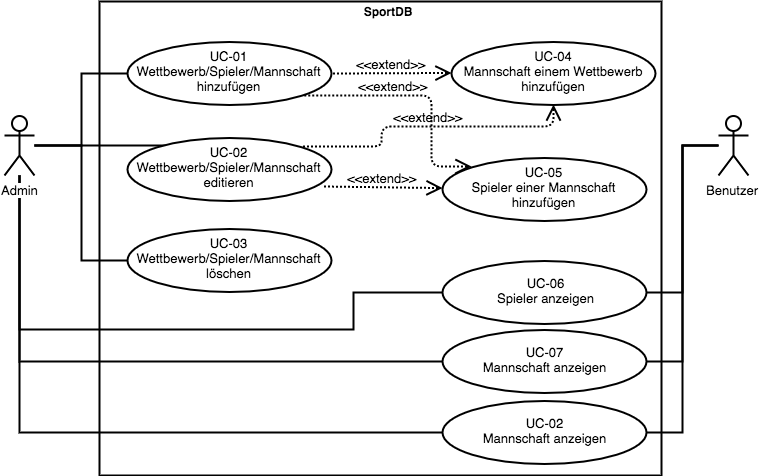
\includegraphics[width=0.9\textwidth]{content/pictures/use_case}
	\label{pic:usecase_diag}
\end{figure}

Aus den groben Anforderungen im Use-Case Diagramm kann man eine Reihe von genauen Anforderungen ableiten.
Diese sind in \ref{tab:anf_seminarverwaltung} beschrieben.


\section{Datenmodell}

Folgendes Datenmodell zu sehen in Abb. \ref{pic:datamodel} ist entstanden. Zu sehen sind die relevanten Modelklassen und ihre Abhängigkeiten zueinander. 
Diese Daten sind durch das CRUD-Framework modifizierbar. Zwischen Wettbewerb und Mannschaft besteht eine One-to-Many Beziehung, genauso wie zwischen Mannschaft und Spieler.




\begin{figure}[htb!]
	\caption{Datenmodell Klassendiagramm}
	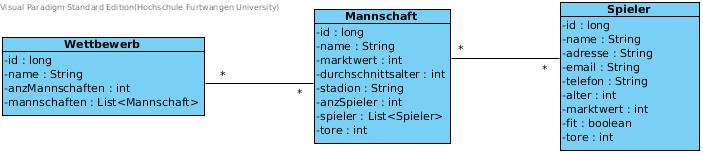
\includegraphics[width=0.9\textwidth]{content/pictures/klassendiagramm_model}
	\label{pic:datamodel}
\end{figure}


